\documentclass{article}

% Language setting
% Replace `english' with e.g. `spanish' to change the document language
\usepackage[english]{babel}

% Set page size and margins
% Replace `letterpaper' with `a4paper' for UK/EU standard size
\usepackage[letterpaper,top=2cm,bottom=2cm,left=3cm,right=3cm,marginparwidth=1.75cm]{geometry}

% Useful packages
\usepackage{amsmath}
\usepackage{graphicx}
\usepackage[colorlinks=true, allcolors=blue]{hyperref}
\usepackage{color}
\usepackage{imakeidx}
\definecolor{mygrey}{gray}{0.75}
\newcommand{\resheading}[1]{{\small \colorbox{mygrey}{\begin{minipage}{0.975\textwidth}{\textbf{#1 \vphantom{p\^{E}}}}\end{minipage}}}}

\title{Hypervisor-PTW}
\author{MicroArch Specification v0.1}

\begin{document}
\maketitle

\begin{abstract}
The PTW module is responsible for translating the virtual address to physical address, the above block diagram represents PTW module working for hypervisor. 
Hypervisor supports two-stage address translation, for any virtual memory access the original virtual address is converted in the first stage byu VS-level address translation, as controlled by vsatp register, into guest physical address. The guest physical address is then converted in the second stage by guest physical address translation as controlled by the hgatp register into a supervisor physical address, the two stage translation are known as VS-stage and G-stage translation 
\end{abstract}

\tableofcontents

\newpage
\section{State Diagram}

%\noindent{\hspace*{\fill}\sphinxincludegraphics{hyperState.png}\hspace*{\fill}}
\begin{center}
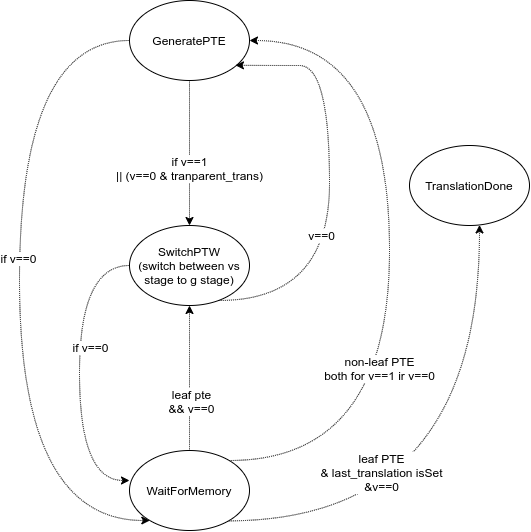
\includegraphics[width=\textwidth]{hyperState.png}
\end{center}


\newpage


\section{Working inside States}

\resheading{\textbf{GeneratePTE}  (for request with V=1) }\\

\textbf{Register used} \\

\textbf{ff\textunderscore request\textunderscore frm\textunderscore core:} the request to ptw module is enqued here.\\

\textbf{rg\textunderscore level\textunderscore VS :}rg\textunderscore level\textunderscore VS : tell which level the VS-stage translation is, this gets sets when request is receive in the subifc\textunderscore request\textunderscore frm\textunderscore core\\

\textbf{rg\textunderscore a\textunderscore VS :}  this is the same register used in the address translation algo description as ‘a’. It is used to store the ppn value albeit the root ppn from the atp.ppn or the intermediate ppn generated during translation by the pte.ppn 

\begin{itemize}


\item Request received
\begin{itemize}
\item Fields inside request
\begin{itemize}	
	\item VA : here for V=1 the VA is the \textbf{GVA}
	\item ATP: here for V=1 the ATP is \textbf{VSSATP}
	\item V: V bit representing which stage of translation this is  V==1 means that its VS-stage translation
\end{itemize}
	
\end{itemize}
	

\item If the translation is a transparent translation then GPA is GVA and save that in \textbf{rg\textunderscore gpa} and set the \textbf{last\textunderscore translation} flag  
\item If it is not a transparent translation then Generate address of PTE from the virtual address and the ppn in the  \textbf{rg\textunderscore a\textunderscore VS} its value is either the ATP.ppn or the  intermediate ppn generated during translation by the pte.ppn 
\begin{itemize}
\item If the \textbf{rg\textunderscore level\textunderscore VS} has the max value which is checked by seeing the mode VS is working on and setting the max value, the atp.ppn value and the va[rg\textunderscore level\textunderscore VS] are concatenated to make the address of PTE
\item If the \textbf{rg\textunderscore level\textunderscore VS}  is less than the max value then \textbf{rg\textunderscore a\textunderscore VS} and va[rg\textunderscore level\textunderscore VS] is used to generate the address of PTE.
\end{itemize}

\item The generated address is the address for the pte, this is the physical address for the VS or c/a \textbf{GPA} 
This GPA need to get translated to host physical address to get the data pointed out by the address GPA the host physical address here is termed as HPA 
\item Save the GPA to a register \textbf{rg\textunderscore gpa}.
\item To get a translation of GPA to HPA we need to switch the ptw to \textbf{G-stage translation} so for a transition of ptw change the state to \textbf{SwitchPTW}.
\end{itemize}

\resheading{\textbf{SwitchPTW  (for request with V=1)}}\\  

\begin{itemize}
\item Check the V bit in the ff\textunderscore req\textunderscore queue, to see which stage of translation the request came from if request came from VS-stage translation then we change the PTW to G-stage translation and vice versa 
\item Save the request inside the ff\textunderscore req\textunderscore queue to ff\textunderscore req\textunderscore of\textunderscore tran\textunderscore gva\textunderscore to\textunderscore hpa, and dequeue the request in ff\textunderscore req\textunderscore queue. This was to done so we can have the main request given to PTW by the TLB miss. 
\item Create a new request with V=0 and enqueue that to ff\textunderscore req\textunderscore que.
\begin{itemize}
\item Fields inside request
\begin{itemize}

\item VA : here we have set V=0 so its a G-stage translation so va is GPA which we get from rg\textunderscore GPA
\item ATP: here for V=0 the ATP is HGATP
\item V: V bit representing which stage of translation this is V==0 meaning G-stage translation 

\end{itemize}
\end{itemize}

\item Also set the rg\textunderscore levels\textunderscore G register using the HGATP.mode value
\item Change the state to generate\textunderscore pte

\end{itemize}

\resheading{\textbf{GeneratePTE  (for request with V=0)}}\\ 

\textbf{Register used} \\

\textbf{ff\textunderscore request\textunderscore frm\textunderscore core:} the request to ptw module is enqued here.\\

\textbf{rg\textunderscore level\textunderscore G :} tell which level the G-stage translation is, this gets sets when request is receive in the subifc\textunderscore request\textunderscore frm\textunderscore core\\

\textbf{rg\textunderscore a\textunderscore G :}  this is the same register used in the address translation algo description as ‘a’. It is used to store the ppn value albeit the root ppn from the atp.ppn or the intermediate ppn generated during translation by the pte.ppn 

\begin{itemize}
\item Request received 
\begin{itemize}
\item Fields inside request
\begin{itemize}

\item VA : here for V=0 the VA is the GPA
\item ATP: here for V=0 the ATP is HGATP
\item V: V bit representing which stage of translation this is  V==0 means that its G-stage translation 
\end{itemize}

\end{itemize}


\item If the translation is a transparent translation/Bare metal translation which can be checked by the HGATP.mode == 0 then copy the value of GPA to rg\textunderscore hpa and since we got the HPA corresponding to GPA we switch the PTW to VS- stage , so to do this change the state to SwtichPTW  
\item Else if it is not a transparent generate address of PTE from the virtual address and the ppn in the  rg\textunderscore a\textunderscore G its value is either the ATP.ppn or the  intermediate ppn generated during translation by the pte.ppn
\begin{itemize}
\item If the rg\textunderscore level\textunderscore G has the max value which is checked by seeing the mode HS is working on and setting the max value, it is atp.ppn value and the va[rg\textunderscore level\textunderscore G] is which are concatenated to make the address of PTE
\item If the rg\textunderscore level\textunderscore G  is less than the max value then rg\textunderscore a\textunderscore G and va[rg\textunderscore level\textunderscore G] is used to generate the address of PTE.
\end{itemize} 

\item The generated address is the address for the pte, this is the physical address for the HS or c/a HPA 
\item Now we want to see which PTE the HPA points to so, we enque the created address to ff\textunderscore memory\textunderscore req with other metadata
\item And finally change the state to WaitForMemory
\end{itemize}


\resheading{\textbf{WaitForMemory  (for request with V=0) }}\\

\begin{itemize}
\item Check the V bit of the request
\item Get the memory value that is the PTE and dequeue the ff 
\item Do permission checks on the PTE
\item FAULTS and TRAP
\item Check if the PTE is leaf PTE or not
\begin{itemize}
\item If non leaf PTE then set the pte.ppn to rg\textunderscore a\textunderscore G and decrement the rg\textunderscore levels\textunderscore G  value by one and change the state to GeneratePTE
\item If it is a leaf PTE then we get the HPA by concatenating the leaf paga pte.ppn with the virtual address of the request i.e. GPA here based on the rg\textunderscore levels\textunderscore G value

\begin{itemize}
\item If it is leaf PTE and last\textunderscore translation flag  is set the set the translation\textunderscore done flag, save the HPA to rg\textunderscore hpa and change the state to TranslationDone

\end{itemize}
\end{itemize}
\item If we get the HPA we got the translation of GPA to HPA in second stage translation so now we will do a lookup for the  PTE in VS Page Table which was earlier pointed out by GPA and since we cannot lookup GPA in pur host machine we got the translation of that address GPA to HPA.
\item We save the HPA inside a reg rg\textunderscore hpa.
\item So to switch the PTW  from Gstage translation to VS stage we change the state to SwitchPTW.
\end{itemize}
 

\resheading{\textbf{SwitchPTW (for request with V=0)}}\\ 

\begin{itemize}
\item Check the V bit in the ff\textunderscore req\textunderscore queue
\item Get the saved request inside ff\textunderscore req\textunderscore of\textunderscore tran\textunderscore gva\textunderscore to\textunderscore hpa and enqueue it into ff\textunderscore req\textunderscore queue 
\item Created request contain the old request given by the TLB
\begin{itemize}
\item Fields inside request
\begin{itemize}

\item VA : here for V=1 the VA is the GVA
\item ATP: here for V=1 the ATP is VSSATP
\item V: V bit representing which stage of translation this is  V==1 means that its VS-stage translation
\end{itemize}
\end{itemize}

\item Now we want to see which PTE the HPA points to so, we enque the rg\textunderscore hpa  address to ff\textunderscore memory\textunderscore req with other metadata
\item Change the state to WaitForMemory.
\end{itemize}

\resheading{\textbf{WaitForMemory (for request with V=1)}}\\ 

\begin{itemize}
\item Check the V bit of the request
\item Get the memory value that is the PTE and dequeue the ff 
\item Do permission checks on the PTE
\item FAULTS and TRAP
\item Check if the PTE is leaf PTE or not
\begin{itemize}
\item If non leaf PTE then set the pte.ppn to rg\textunderscore a\textunderscore VS and decrement the rg\textunderscore levels\textunderscore VS  value by one and change the state to GeneratePTE
\item If it is a leaf PTE then we get the final GPA by concatenating the leaf pte pte.ppn with the virtual address of the request i.e. GVA here based on the rg\textunderscore levels\textunderscore VS value and we set flag last\textunderscore translation 
\end{itemize}
\item Change the state to SwitchPTE 
\end{itemize}
\newpage
\resheading{\textbf{Translation\textunderscore done}}\\
\begin{itemize}
\item Dequeue the ff\textunderscore req\textunderscore queue 
\item Send the response to tlb with GVA, HPA,  GPA,  HPA[p] GPA[p]
\begin{itemize}
\item GVA we can get from ff\textunderscore gva\textunderscore to\textunderscore hpa\textunderscore translation 
\item HVA we get from rg\textunderscore hpa
\item GPA we get from rg\textunderscore gp
\end{itemize}

\end{itemize}

\newpage

\section{Block Diagram Explanation}
Below is the description for the block diagram for PTW-hypervisor.\\ \\
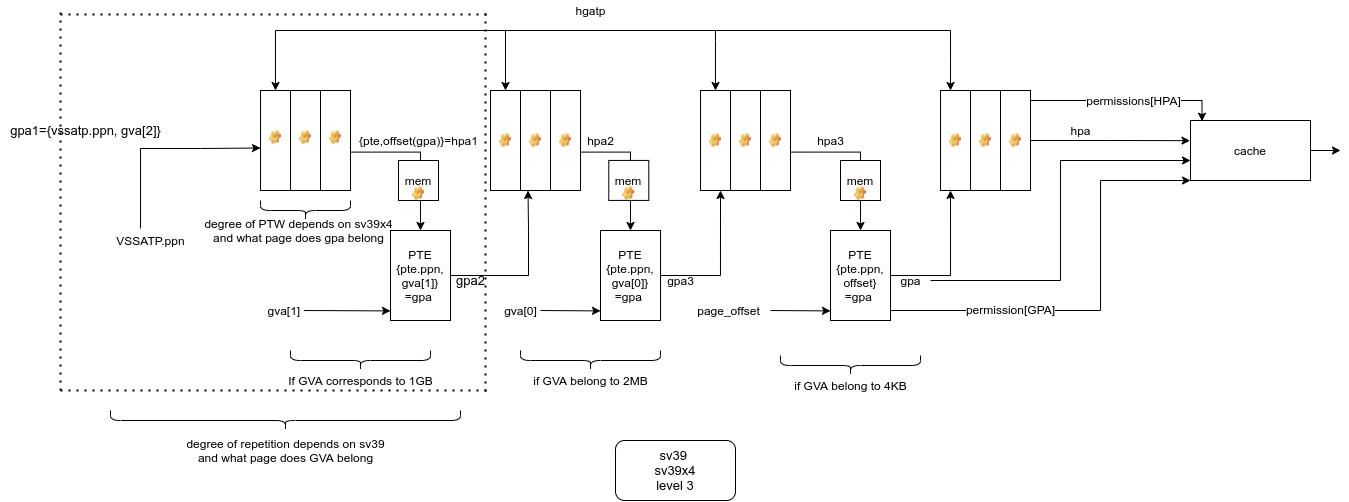
\includegraphics[width=\textwidth]{hypervisor.png}
\\ \\
Note for a n-level ptw, n is bounded by two things first one is the virtualization mode the ptw is happening which bounds the max value of n and the page that virtual address belongs to which tell at which level the ptw will get the ppn from for example for a sv39 mode where the virtual address belongs to 2mib page then the ptw will get the ppn from 2-level ptw \\

Description below assumes that the  GVA and GPA belong to 4KiB page, and the VS mode is sv39 and HS mode is sv39x4
The virtual address generated by the core in VS mode need to get translated to physical memory 
\begin{enumerate}
\item Initially, the core is in vs mode so the virtual address GVA will first get translated to GPA. the value of GPA is the concatenation of vssatp.ppn and gva[2].
\item Gpa is then translated to hpa usig hgatp csr, by a 3-level page table walk. This PTW is the G-stage translation of gpa to hpa 
\item The final hpa that is the translation of gpa is created by concatenating the pte.ppn of last level ptw ,in gstage translation  and offset which we get from the 12 LSB of GPA 
\item This HPA is a physical address of GPA in the host machine so a memory access is done using this address to figure out the PTE the GPA points to.
\item The response of memory access is a pte and the ppn is concatenated with gva[1] to get the gpa2. 
\item The above step from step 2 to 5 are 1st level ptw of Vs-stage translation, so the steps 2-5  are repeated 2 more times with appropriate gpa and gva values to for a 3 level PTW in vs mode of translating the gva to gpa, after we get the final gpa a final G-stage translation is done to converte the gpa to hpa and appropriate values are send to response of the ptw which mainly consist of requested GVA whose translatio nis requested, then the GPA along with its permissions bits which are used for the final g-stage translation and hpa along with its permission bits that we get at end of whole ptw 
\end{enumerate}

\newpage

\section{Interface Explanation}
Below is the description for the block diagram for PTW-hypervisor.\\ \\
\begin{center}
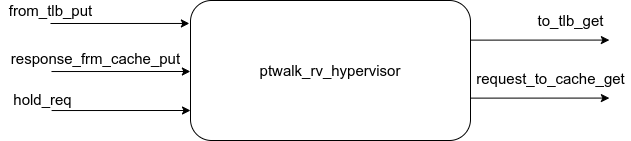
\includegraphics[width=0.8\textwidth]{hyperInterface.png}
\end{center}


\begin{itemize}

\item \textbf{from\textunderscore tlb\textunderscore put}: Put interface, i.e input port. This interface is used to get the incoming request from TLBs
\item \textbf{to\textunderscore tlb\textunderscore get}: Get interface, i.e output port. This interface is used to send the response of ptwalk to TLBs
\item \textbf{response\textunderscore frm\textunderscore cache\textunderscore put}: Put interface, i.e. input port. This interface in used to get response of the memory request that is send by the PTWALK module to cache
\item \textbf{hold\textunderscore req} : Put interface, i.e. input port. When the core requests a memory it sends out a address to Dcache, Dcache enqueues the request to ptwalk as well as TLB hold\textunderscore req is used to input the request for which there is a TLB miss so that after the ptwalk is completed ptwalk can enqueue the request to cache and cache can replay the memory request.
\item \textbf{request\textunderscore to\textunderscore cache\textunderscore get}: Get interface, i.e output port. This sends out the request to cache.
\end{itemize}

\newpage

\section{Data Structure used description}

To be included after 1st iteration of code.....



\bibliographystyle{alpha}
\bibliography{sample}

\end{document}